% TikZ: Menulis huruf T dengan titik-titik koordinat
% Aktivitas kelas: gambar huruf dari pasangan (x, y)
\documentclass[tikz]{standalone}
\usepackage{amsmath}
\usepackage{amssymb}
\definecolor{bg}{HTML}{171D2B}
\definecolor{gridc}{HTML}{1E293B}
\definecolor{aksen}{HTML}{F7B538}
\begin{document}
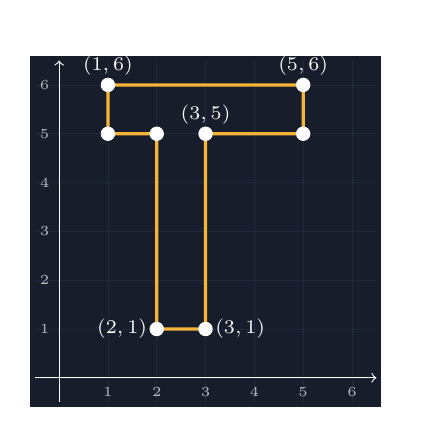
\begin{tikzpicture}[x=0.62cm, y=0.62cm]
  % Latar gelap
  \fill[bg] (-0.6,-0.6) rectangle (6.6,6.6);

  % Grid halus
  \begin{scope}
    \clip (-0.5,-0.5) rectangle (6.5,6.5);
    \foreach \i in {0,...,6} {
      \draw[gridc, very thin] (\i,-0.5) -- (\i,6.5);
      \draw[gridc, very thin] (-0.5,\i) -- (6.5,\i);
    }
  \end{scope}

  % Sumbu
  \draw[white, ->] (-0.5,0) -- (6.5,0) node[below right, text=white, font=\footnotesize] {$x$};
  \draw[white, ->] (0,-0.5) -- (0,6.5) node[above left, text=white, font=\footnotesize] {$y$};
  \foreach \i in {1,...,6} {
    \node[below, text=white!70!bg, font=\tiny] at (\i,0) {\i};
    \node[left,  text=white!70!bg, font=\tiny] at (0,\i) {\i};
  }

  % Huruf T dari titik-titik
  \draw[aksen, very thick, rounded corners=2pt]
    (1,6) -- (5,6) -- (5,5) -- (3,5) -- (3,1) -- (2,1) -- (2,5) -- (1,5) -- cycle;

  \foreach \p in {(1,6),(5,6),(5,5),(3,5),(3,1),(2,1),(2,5),(1,5)}
    \fill[white] \p circle (2.6pt);

  % Label koordinat beberapa titik
  \node[above, text=white, font=\scriptsize] at (1,6) {$(1,6)$};
  \node[above, text=white, font=\scriptsize] at (5,6) {$(5,6)$};
  \node[right, text=white, font=\scriptsize] at (3,1) {$(3,1)$};
  \node[left,  text=white, font=\scriptsize] at (2,1) {$(2,1)$};
  \node[above, text=white, font=\scriptsize] at (3,5) {$(3,5)$};
\end{tikzpicture}
\end{document}
